\section{Main contributions}\label{contributions}
The main contribution of this thesis is the theoretical foundation of a new approach to UI development with a UI framework. A proof of concept demonstrates the major theoretical contributions. On a larger scale this thesis contributes to the fight against accidental complexity in software development.

\subsection{Methods}\label{usecases}
We chose to follow a process including the following points in order to explore possible answers and solutions to the thesis.

\subsubsection{Conceptual analysis of user interfaces}
Through observation of the typical usage patterns of user interfaces we can derive coarse business requirements of the UI framework. These serve as foundation for further requirements engineering.

\subsubsection{Definition of major design goals}
Major design goals of the UI framework are directly influenced by non-functional requirements. We consider the broader scope of UI development in order to obtain those. This includes analysis of:

\begin{enumerate}
  \item the development process of UIs with web technologies
  \item contemporary frameworks and tools for UI development that enjoyed wide and rapid adoption
  \item contemporary frameworks and tools for UI development that failed
\end{enumerate}

By following what tools in \textbf{2} did right and avoiding the mistakes of tools in \textbf{3}, we define a set of design goals that the proof of concept should adhere to.

\subsubsection{Definition of the proof of concept}
The section defines the artifact that can be used to create UIs. The proof of concept should demonstrate the viability of the thesis.

\subsubsection{Definition of the development process}
The proof of concept is a software artifact and is developed with respect to current engineering best practices.

\subsubsection{Definition of real world use cases}
By defining real world applications for the UI framework, we discover user roles and user stories.

\subsubsection{Implementation of proof of concept driven by use cases}
The UI framework is developed incrementally use case by use case. The major design goals are respected.

\subsubsection{Evaluation of proof of concept}

\subsubsection{Conclusion of approach to reduce accidental complexity}

\subsection{Conceptual analysis of user interfaces}
For a system to be useful, it has to interact with its environment. These interactions happen through multiple types of interfaces, which are used by two types of users. The users are either other systems or human users.
The interfaces for human users (user interfaces) have typical characteristics,
By observing the usage of a user interface by the user we can analyze the main characteristics. A typical scenario of UI usage is browsing a website. What does the user do while browsing a website? It is typically one of two things: he either reads or clicks.

\textbf{Reading} a website is equivalent to data \textbf{querying}. The user \textbf{querying} data

The usage of a UI by a user consists of either \textbf{reading} or \textbf{interacting}. In terms of systems we can call them \textbf{querying} or \textbf{interacting} respectively.
\begin{enumerate}
  \item Query: The user is able to retrieve information from the UI by looking at it
  \item Interacting: The user is able to interact with the UI
\end{enumerate}

The development of the UI framework is driven by the implementation of these two capabilities.

\subsection{Design goals}
Following design goals should be met by the UI framework.

\subsubsection{Play nicely with others}\label{usecases}
The most important design goal is to play nicely with others. We achieve that by conforming to web standards and making use of existing and established tooling. This design goal drove the choice of JSON-LD as serialization format for linked data.

JSON-LD allows us to stay compatible with all tools consuming and producing JSON.

\subsubsection{Straightforward upgrade path}\label{usecases}
By playing nicely with others, the UI framework is able to provide an upgrade path to already existing APIs.

\subsubsection{Customizability}\label{usecases}

\subsubsection{Developer ergonomics}\label{usecases}

\subsection{Proof of concept}
I define two real-world use cases that cover the two main capabilities of \textbf{rendering data} and \textbf{user interaction}. Each of those use cases are split up into user stories that can be implemented separately. This ensures that the design goals are met and all user roles are considered.

\subsection{Use Case 1: Apartment}\label{usecases}
For the user to be able to query data, the UI has to render it.

The first use case describes a scenario in home automation. Several thermometers in several rooms in an apartment send the current temperature to a server. The goal is to develop a UI that displays apartments, rooms, and thermometers and temperatures in a sensible manner.

\begin{figure}[!htb]
  \center{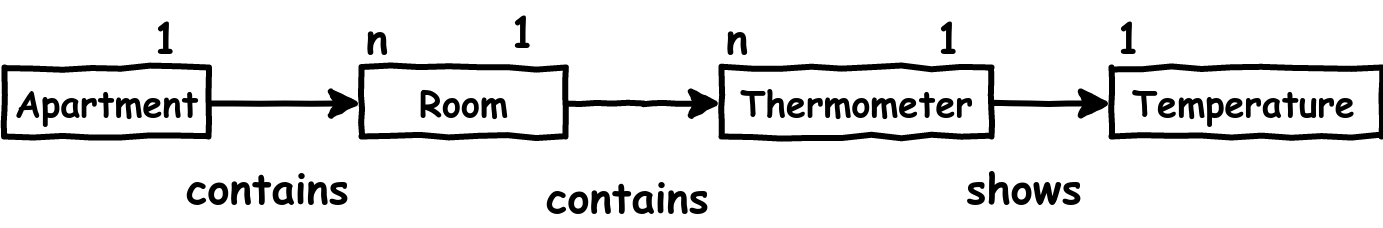
\includegraphics[width=100]
    {images/iot.png}}
  \caption{\label{fig:my-label} Data model of the kanban board use case.}
\end{figure}

\begin{table}
\begin{center}
\begin{tabular}{ |c|l| }
 \hline
 ID & Story title \\
 \hline
 S01 & As landlord I want to overview my apartments \\
 S02 & As landlord I want to overview all rooms of an apartment \\
 S03 & As landlord I want to overview thermometers of room \\
 S04 & As landlord I want to overview the measurement data of a thermometer \\
 S05 & As UI developer I want to present all available data without spending any development time \\
 S06 & As UI developer I want to be able to customize the UI in order to improve it incrementally \\
 \hline
\end{tabular}
\caption{User stories of a client that consumes a home automation API}
\end{center}
\end{table}

\subsection{Use Case 2: Kanban Board}\label{usecases}

\begin{figure}[!htb]
  \center{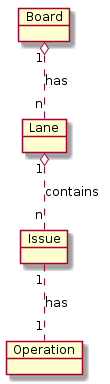
\includegraphics[width=100]
    {images/kanban.png}}
  \caption{\label{fig:my-label} Data model of the home automation use case.}
\end{figure}

\begin{table}
\begin{center}
\begin{tabular}{ |c|l| }
 \hline
 ID & Story title \\
 \hline
 S01 & As project manager I want to overview all projects \\
 S02 & As project manager I want to overview all issues of a project \\
 S03 & As project manager I want to see the status of an issue \\
 S04 & As project manager I want to change the status of an issue \\
 S05 & As project manager I want to create new issues \\
 S06 & As project manager I want to remove issues \\
 S07 & As UI developer I want to present all available data without spending any development time \\
 S08 & As UI developer I want to be able to customize the UI in order to improve it incrementally \\
 \hline
\end{tabular}
\caption{User stories of a simple software project management tool}
\end{center}
\end{table}

\subsection{Base hypermedia vocabulary}\label{basevocab}

\subsection{UI rendering}\label{genericrendering}

This paragraph focuses on presentation of data by rendering UI components in the context of web development.


\subsubsection{Rendering UIs using linked data}\label{linkeddatarendering}

\begin{figure}[!htb]
  \center{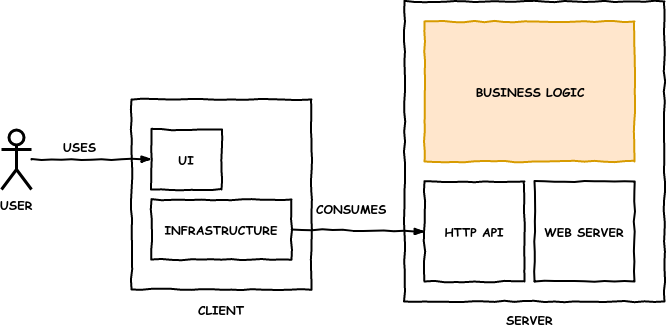
\includegraphics[width=380]
    {images/ui-dev.png}}
  \caption{\label{fig:my-label} Solely the server contains business logic.}
\end{figure}

\subsubsection{Pluggable domain rendering}\label{domainrendering}

\begin{figure}[!htb]
  \center{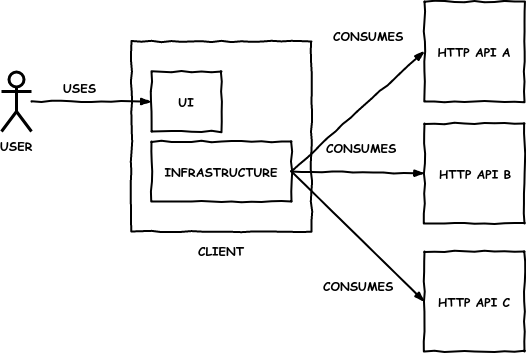
\includegraphics[width=380]
    {images/client-instances.png}}
  \caption{\label{fig:my-label} The client is decoupled from any API and is able to consume different APIs.}
\end{figure}

\begin{figure}[!htb]
  \center{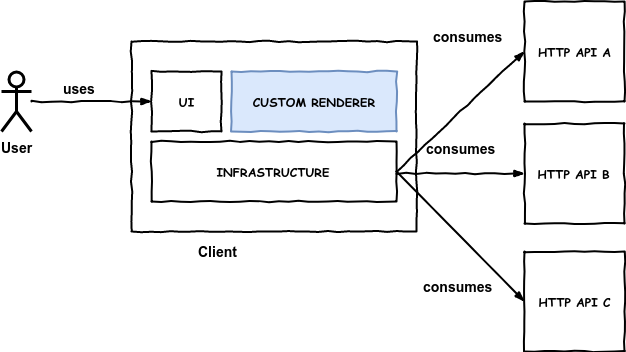
\includegraphics[width=380]
    {images/ui-dev-custom-renderer.png}}
  \caption{\label{fig:my-label} Custom renderers provide the ability to render linked data types. By avoiding hard coding business logic into the client the coupling to the server is still lose.}
\end{figure}

\subsection{User interaction}\label{interaction}

\subsubsection{Task based computing}\label{interaction}
TODO three types of operations:

inline operations
supported operations for all of the resource's types
supported operations for the supported property, where the resource is an object of said property

\subsubsection{CQRS}\label{interaction}
